%% Template article for Elsevier's document class `elsarticle'
%% with numbered style bibliographic references
\documentclass[preprint,12pt]{elsarticle}

% remove preprint footnote
\makeatletter
\def\ps@pprintTitle{%
 \let\@oddhead\@empty
 \let\@evenhead\@empty
 \def\@oddfoot{\centerline{\thepage}}%
 \let\@evenfoot\@oddfoot}
\makeatother


\usepackage{setspace}
\doublespacing

\usepackage{hyperref} % auto detect ref type
\usepackage{natbib}
\setcitestyle{authoryear}

%% Use the option review to obtain double line spacing
%% \documentclass[preprint,review,12pt]{elsarticle}

%% Use the options 1p,twocolumn; 3p; 3p,twocolumn; 5p; or 5p,twocolumn
%% for a journal layout:
%% \documentclass[final,1p,times]{elsarticle}
%% \documentclass[final,1p,times,twocolumn]{elsarticle}
%% \documentclass[final,3p,times]{elsarticle}
%% \documentclass[final,3p,times,twocolumn]{elsarticle}
%% \documentclass[final,5p,times]{elsarticle}
%% \documentclass[final,5p,times,twocolumn]{elsarticle}

\usepackage{graphicx}
\usepackage{amssymb}
\usepackage{amsmath}
\usepackage{enumerate}
\usepackage{caption}
\usepackage{textcomp}    % for Hawaii characters
%\usepackage{listings}
%\lstset{language=R}
\usepackage[T1]{fontenc}  % tilde in middle in lstlisting
\usepackage[formats]{listings}
\lstset{language=R,
		basicstyle=\ttfamily,
		columns=fixed,
		basewidth=0.5em,
		literate={~}{{$\sim$}}1
		}

\biboptions{comma,round}

% shortcuts
\newcommand{\bbeta}{\boldsymbol{\beta}}
\newcommand{\blambda}{\boldsymbol{\lambda}}
\newcommand{\T}{\intercal}
\newcommand{\bS}{\mathbf{S}}
\newcommand{\bQ}{\mathbf{Q}}
\newcommand{\bSigma}{\boldsymbol{\Sigma}}
\newcommand{\bm}{\boldsymbol}  % bold maths symbols
\newcommand{\tl}{\tilde{\lambda}}   % thinned little lambda
\newcommand{\tL}{\tilde{\Lambda}}  % thinned big lambda

% RJC 09/08/2019 Added shortcuts for Hawaiian words
\newcommand{\akepa}{\textquotesingle\={a}kepa}  % adds Hawaiian diacritical marks
\newcommand{\Akepa}{\textquotesingle\={A}kepa}  % adds Hawaiian diacritical marks
\newcommand{\hawaii}{Hawai\textquotesingle i}   % adds Hawaiian diacritical marks
\DeclareMathOperator*{\argmax}{arg\,max}  % * means _ puts thing beneath operator

\begin{document}
\begin{frontmatter}
\title{One-stage point transect distance sampling using iterated integrated nested Laplace approximations}

%% use the tnoteref command within \title for footnotes;
%% use the tnotetext command for the associated footnote;
%% use the fnref command within \author or \address for footnotes;
%% use the fntext command for the associated footnote;
%% use the corref command within \author for corresponding author footnotes;
%% use the cortext command for the associated footnote;
%% use the ead command for the email address,
%% and the form \ead[url] for the home page:
%%
%% \title{Title\tnoteref{label1}}
%% \tnotetext[label1]{}
%% \author{Name\corref{cor1}\fnref{label2}}
%% \ead{email address}
%% \ead[url]{home page}
%% \fntext[label2]{}
%% \cortext[cor1]{}
%% \address{Address\fnref{label3}}
%% \fntext[label3]{}


%% use optional labels to link authors explicitly to addresses:
%% \author[label1,label2]{<author name>}
%% \address[label1]{<address>}
%% \address[label,2]{<address>}

% RJC 09/08/2019 Added co-authors and affiliations. Note that I used \affil[]{} instead of \address[]{}
\author[1,*]{Andrew E Seaton}
\author[1,2]{Richard J Camp}
\author[3]{Finn Lindgren}
\author[1]{Janine B Illian}
\author[1]{David L Borchers}
\author[1]{David L Miller}      % Ask about co-authoring the manuscript
\author[1]{Len Thomas}          % Ask about co-authoring the manuscript
\author[1]{Stephen T Buckland}  % Ask about co-authoring the manuscript
\author[4]{Steve J Kendall}     % It is Steve's data we are using and I have already mentioned this manuscript to him.

%\address{Centre for Research into Ecological \& Environmental Modelling and School of Mathematics \& Statistics, University of St Andrews, St Andrews, Fife, Scotland}
\address[1]{Centre for Research into Ecological \& Environmental Modelling and School of Mathematics \& Statistics, University of St Andrews, St Andrews, Fife, Scotland}
\address[2]{U. S. Geological Survey, Pacific Island Ecosystems Research Center, P.O. Box 44, \hawaii{} National Park, HI 96718, U.S.A.}
\address[3]{School of Mathematics, University of Edinburgh, Edinburgh, Scotland}
\address[4]{U. S. Fish and Wildlife, Big Island National Wildlife Refuge Complex, 60 Nowelo St., Suite 100, Hilo, HI  96720, U.S.A.}
\address[*]{Correspondence: Andrew E Seaton, Email: aes22@st-andrews.ac.uk}

\begin{abstract}
A New Abstract Goes Here   
\end{abstract}

%\begin{keyword}
%Distance sampling \sep Stochastic partial differential equations \sep Integrated nested Laplace approximation \sep Generalized additive model
%\end{keyword}
\end{frontmatter}

\section{Introduction}

The estimation of the size and spatial distribution of wild populations of animals is a critical objective within ecology and conservation \citep{schwarz_estimating_1999}. Here we present an analysis of wildlife survey data collected on a critically endangered Hawaiian forest bird that aims to meet this objective.  The Hawaiian \akepa{} is an endemic species whose population declined dramatically during the 20th century [[cite??]].  The remaining population is the focus of sustained conservation efforts and monitoring is required to inform decision-makers about changes in the overall abundance and spatial distribution.  This information is critical when making decisions about conservation strategies.  However, answering these questions presents many statistical challenges.  

Firstly, as in many ecological surveys, it is impossible to undertake a census.  The existing population numbers in the thousands and lives in dense forest where logistical and ecological challenges mean a census is not feasible.  For this reason, a monitoring survey must sub-sample in space and time in some way.  For the \akepa{} this takes the form of the Hawaii Forest Bird Survey (HFBS) \citep{scott_HFBS_1986} which is a large-scale, quantitative survey of Hawaiian forest birds.  Annual surveys of the \akepa{} study-region consist of survey points located along randomly located transects.    

Secondly, even at sampled locations, detectability of animals is uncertain.  The \akepa{} survey attempts to estimate detectability using a distance sampling approach \citep{buckland_distance_2015} where for each observation the distance to the observer is recorded.  A parametric form of detection function is assumed to decay with increasing distance and is estimated from the observed distances.  Because of this, answering questions related to the abundance and spatial distribution must involve the estimation of a complex observation process.  

Thirdly, due to the spatial sub-sampling, a key aim of the analysis is the generation of spatial predictions.  However, as is the case in many species distribution models, we usually have reason to believe there are drivers of the spatial distribution for which we have no explanatory covariates.  For the \akepa{} this takes the form of a north-south gradient that has been investigated but for which no clear-cut explanatory cause has been found [[cite here?]].  From a statistical perspective this suggests the use of spatially-structured random effects to account for the missing covariates.

Fourthly, the resulting statistical model is complex and it is therefore challenging to effectively communicate the results of the analysis to non-statistically trained stakeholders such as conservation managers and policy officers.  In particular we note the challenge of communicating uncertainty in maps of predicted animal density.

In this paper we present an analysis that seeks to address each of these issues by presenting

\begin{enumerate}[(i)]
	\item A model-based spatial point process perspective on point transect distance sampling, representing the observation model as a thinning probability function.
	\item A one-stage approximate Bayesian approach to inference to simultaneously estimate the observation model and spatial distribution.  This is based on iterated model fits using integrated nested Laplace approximations (INLA) \citep{rue_approximate_2009}.
	\item A computationally efficient Gaussian Markov random field (GMRF) spatial effect based on a stochastic partial differential equation approach \citep{lindgren_explicit_2011} to account for missing covariates.
	\item An approach to model evaluation and communication based on sampling from the joint posterior of all model parameters and excursions methods \citep{bolin_excursion_2015} for investigating uncertainty in spatial predictions.
\end{enumerate}

We note that these challenges are generic to many types of wildlife survey data, not only the \akepa{} survey, and can be addressed by a range of possible statistical approaches.  Our analysis here is one possible choice of approach and throughout the remainder of the paper we will highlight differences with existing approaches. It is important to note that we do not claim any overall superiority of this approach over others, although we do highlight some areas for which we believe our approach provides a natural setting for addressing the issues above.  We demonstrate several novel contributions to the problem of species distribution modelling under imperfect detection.  In particular, the point process perspective with incomplete location information, the one-stage approximate Bayesian inference strategy and focus on communicating uncerainty in spatial predictions using excursions are innovations in this area.  We also note that although we use a Bayesian approach, maximum-likelihood frameworks could also have been used.  Finally, we note that many of the themes addressed in this paper apply beyond the field of spatial ecology and will be of interest to the spatial statistics community in general, particularly for applications with complex observation models of latent processes and where spatial predictions are a key output of the analsyis.

The rest of the paper proceeds as follows:  (i) we describe in detail the \akepa{} study-region and survey design; (ii) we present the perspective of distance sampling as a thinned point process; (iii) we describe the GMRF random effect and iterated INLA fitting procedure; (iv) we present the results of the analysis and discuss model evaluation and communication.

\section{Study design}

The \hawaii{} \akepa{} (hereafter \akepa{}; \textit{Loxops coccineus}; nomenclature according to \citealp{usfws_akepa_1970}) is an internationally and federally endangered Hawaiian honeycreeper (\citealp{usfws_akepa_1970, birdlife_akepa_2016}) that is endemic to \hawaii{} Island, USA.  Large-scale, quantitative surveys of Hawaiian forest birds and their habitat commenced in the mid-1970s through the Hawaii Forest Bird Survey (HFBS) \citep{scott_HFBS_1986}. Information from the HFBS was used to update the listing and delisting of endangered species, and establish preserves that coincided with native bird hotspots, including Hakalau Forest National Wildlife Refuge on \hawaii{} Island (hereafter Hakalau) that was the first wildlife refuge with the primary purpose to protect, conserve and manage native forests for threatened and endangered bird and plant species. Due to the broad-scale coverage and robust design HFBS has become the baseline to determine changes in bird species distributions, population sizes and trends in density patterns over time.

During the 20th century \akepa{} declined dramatically due to habitat modification \citep{scott_HFBS_1986, pratt_avifaunal_1994},  mosquito-transmitted avian diseases \citep{pratt_avifaunal_1994, atkinson_wildlife_1995}, introduced predators \citep{lepson_akepa_1997}, and food resources competitors \citep{lepson_akepa_1997}. \Akepa{} has a global abundance of approximately 16,200 (95\%CI 10,000\textendash25,200) birds that has been restricted to five spatially distinct populations \citep{judge_akepa_2018}. Hakalau supports the largest \akepa{} population that in 2012 was estimated at more than 11,000 birds \citep{camp_statespace_2016}. Maintaining and expanding the \akepa{} population at Hakalau is a primary conservation concern. Moreover, having unbiased and precise abundance estimates are required by land and resource managers for evaluating management actions and establishing management planning, and policy makers for decision-making processes.

\subsection{Study area and sampling method}

[[Need to update this and the figure with the extended data area]]

Hakalau was established in 1985 to conserve 15,390-ha of montane forest habitat for native forest birds and rainforest plants. Annual forest bird surveys were initiated in 1987 to determine population status and track trends in abundance. Survey points were established along 15 transects following a systematic, random design with points approximately 150 m apart on transects located either 500 or 1,000 m apart. Following \cite{camp_population_2010, camp_statespace_2016}, we restrict our study area to the 3,061 ha open-forest stratum of Hakalau.  The open-forest stratum was previously heavily grazed, and since the removal of cattle in 1988 regeneration has proceeded naturally \citep{maxfield_hakalau_1998}. To the north the study area follows the refuge boundary while to the east it is bounded by a fence line (Fig. \ref{fig:2002studyareapointspt}). The southern boundary was modified from \cite{camp_population_2010} to exclude the non-sampled forested portion of their study area. The west side of the study area is bounded by pasture that is dominated by grass and is unsuitable habitat for \akepa.

\begin{figure}
	\centering
	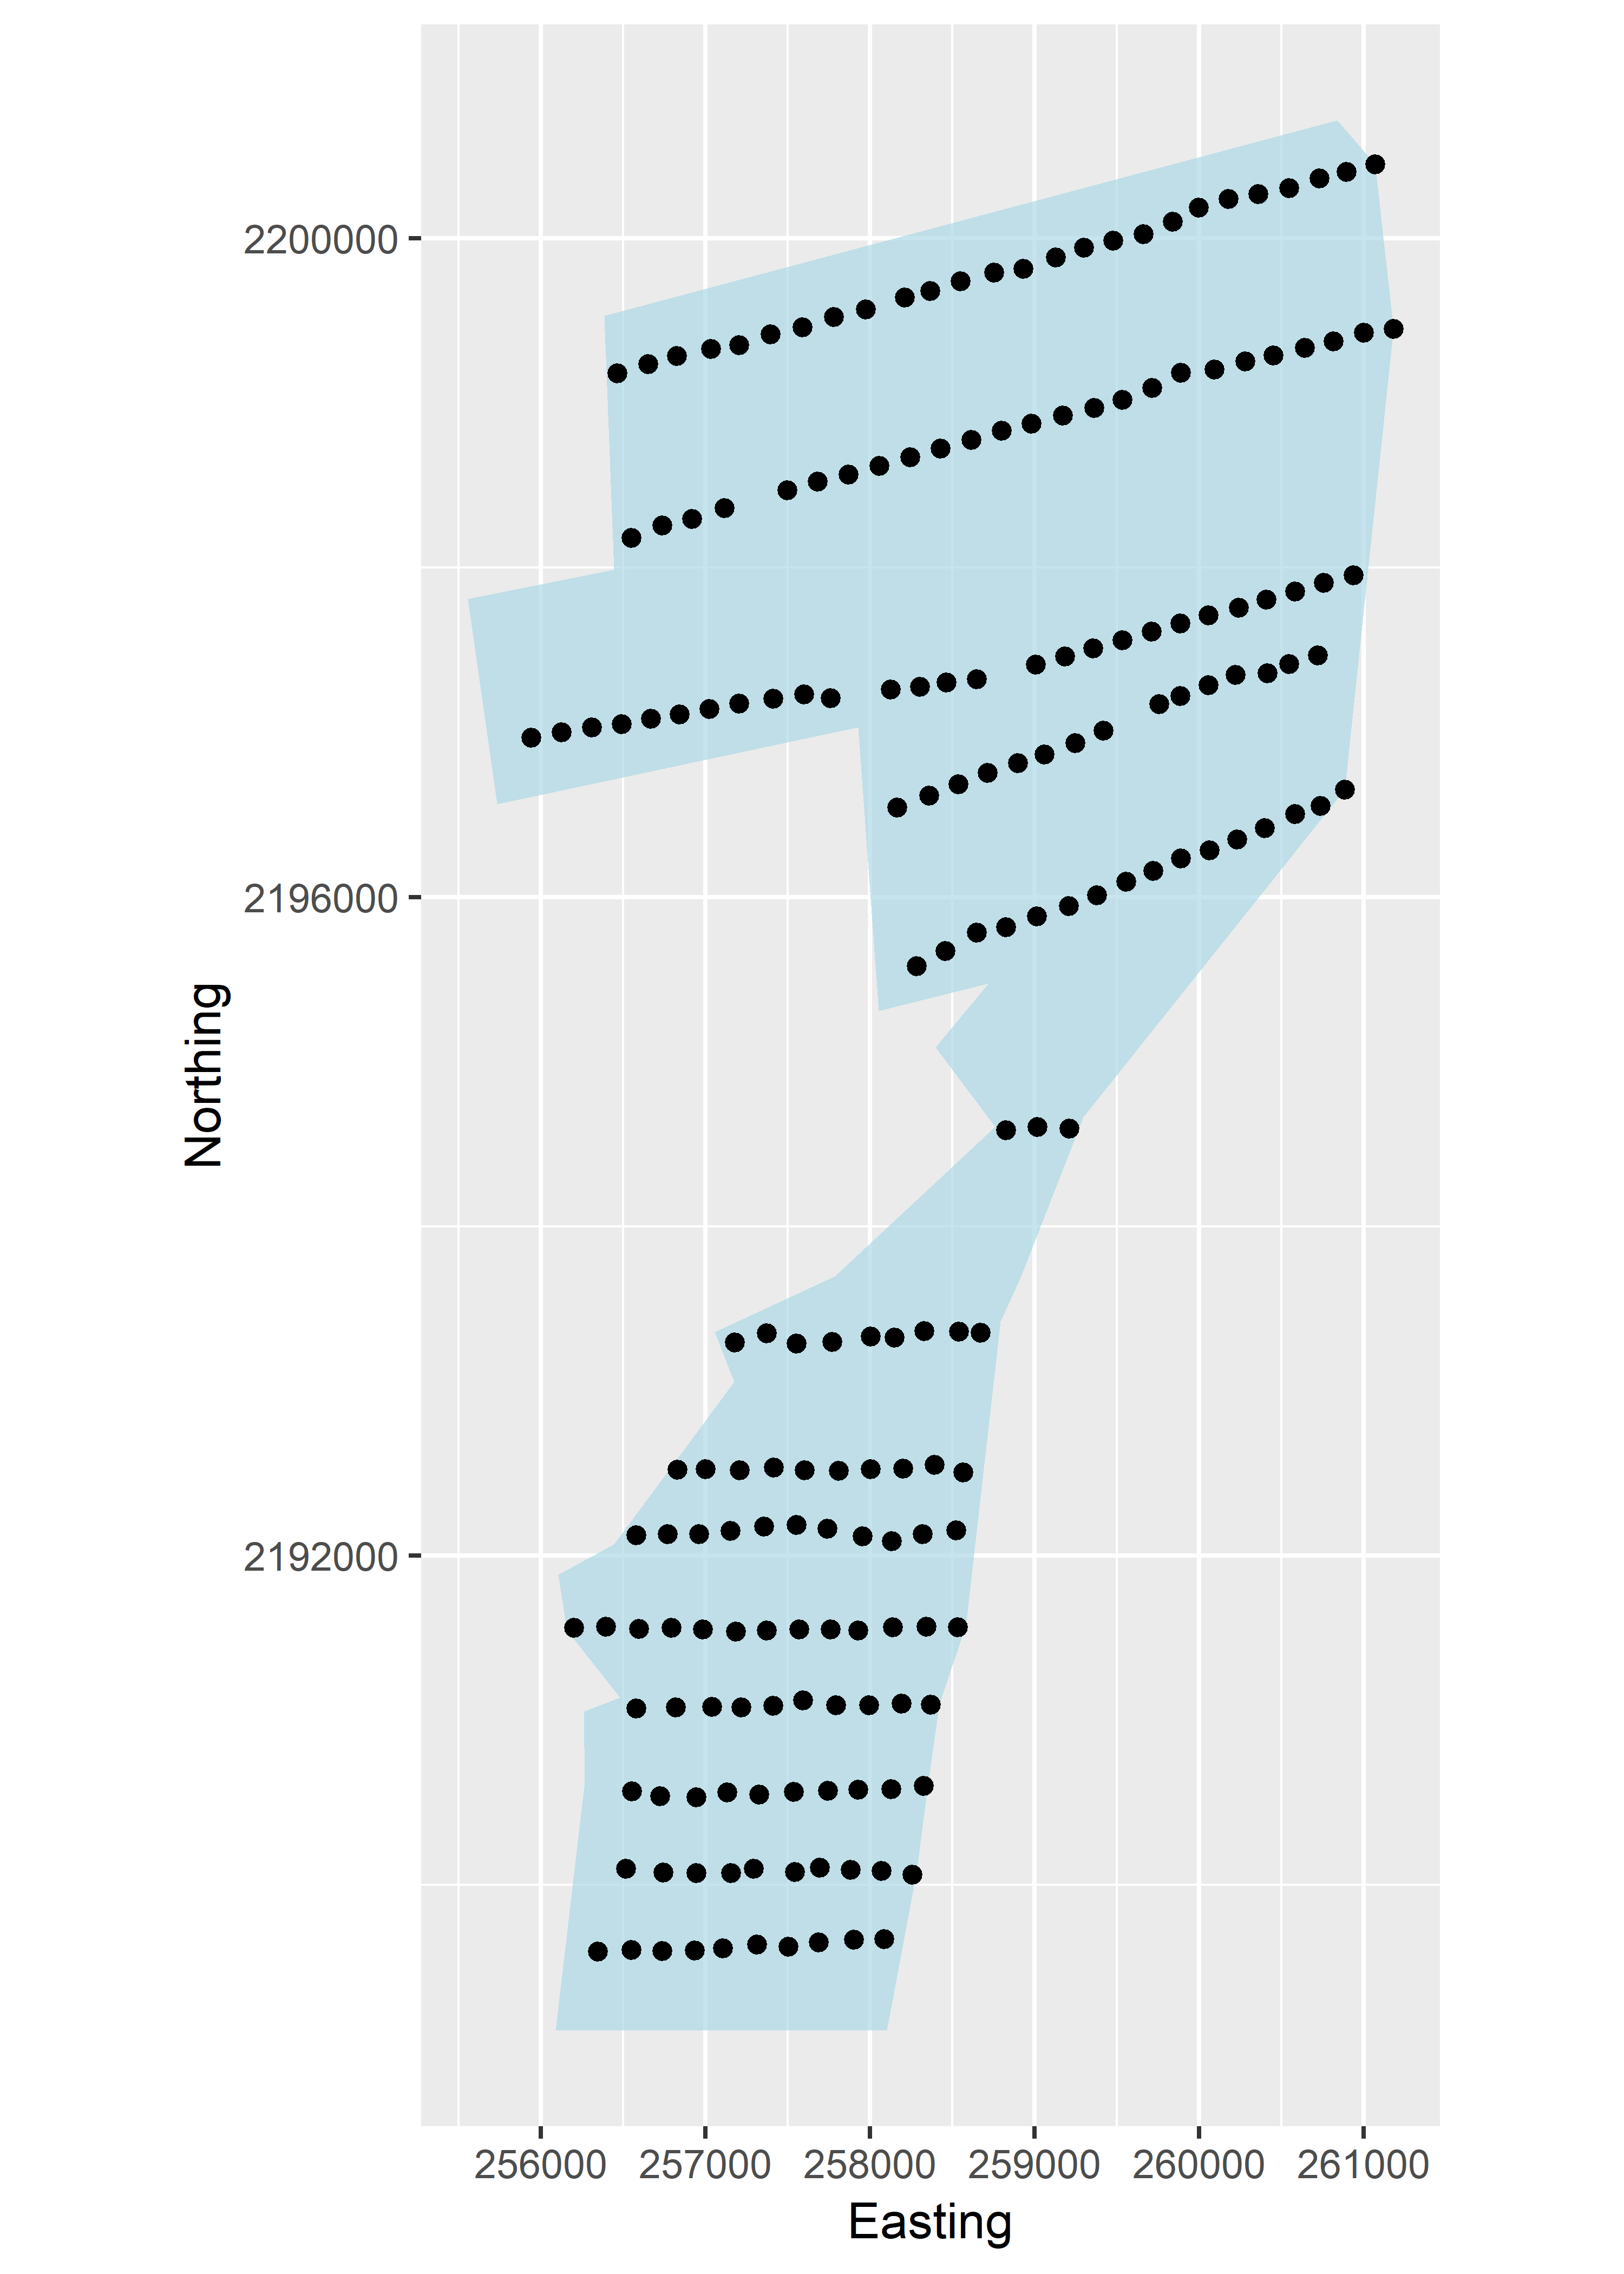
\includegraphics[scale=0.5]{figures/2002studyareapoints_pt}
	\caption{Study area (light blue) showing the 2002 survey points (black dots) in Hakalau Forest National Wildlife Refuge, \hawaii{} Island.}
	\label{fig:2002studyareapointspt}
\end{figure}

Surveys used point-transect methods, recording horizontal distances from survey points to individually detected birds. Surveys commenced at dawn and continued until 11:00 or halted when weather conditions exceeded prescribed conditions that hindered detecting birds (light rain, and wind and gust strength \textgreater Baufort scale 3). During 8-min counts trained observers recorded the species, exact distance to the nearest meter and detection type for each bird detected, along with the sampling conditions cloud cover, rain, wind strength, gust strength, and time of day each point was surveyed.   \cite{camp_population_2010,camp_statespace_2016} provide a detailed description of Hakalau, the open-forest study area and the bird surveys.

\subsection{Data description}
[[ Need to update this with extended data ]]

For the purposes of our analysis we selected a single survey from the \akepa{} time series that contained on broad sampling of the study area with sufficient numbers of detections to estimate detectability. In 2002, 289 points were sampled using point-transect distance sampling methods within the 3,061 ha open-forest study area of Hakalau (Fig. \ref{fig:2002studyareapointspt}). 276 \akepa{} were detected on 121 point transects. The number of detections within each sampling unit ranged from zero to 6. 


\section{Distance sampling as a thinned point process}



\section{Iterated INLA}

\begin{itemize}
	\item mini lit review - communicating uncertainty in spatial models w random effects
	(should this really be here??  Think about moving)
\end{itemize}

\section{GMRF + SPDE}

\section{Results}

\section{Model Evaluation}

\begin{itemize}
	\item Posterior sampling
	\item Barplot for random effect
	\item Excursions
\end{itemize}

\section{Discussion}

Discuss wisely

\bibliographystyle{chicago}
\bibliography{paper}

\end{document}